%%%%%%%%%%%%%%%%%%%%%%%%%%%%%%%%%%%%%%%%%
% Focus Beamer Presentation
% LaTeX Template
% Version 1.0 (8/8/18)
%
% This template has been downloaded from:
% http://www.LaTeXTemplates.com
%
% Original author:
% Pasquale Africa (https://github.com/elauksap/focus-beamertheme) with modifications by 
% Vel (vel@LaTeXTemplates.com)
%
% Template license:
% GNU GPL v3.0 License
%
% Important note:
% The bibliography/references need to be compiled with bibtex.
%
%%%%%%%%%%%%%%%%%%%%%%%%%%%%%%%%%%%%%%%%%

%----------------------------------------------------------------------------------------
%	PACKAGES AND OTHER DOCUMENT CONFIGURATIONS
%----------------------------------------------------------------------------------------

\documentclass[aspectratio=169]{beamer}

\usetheme{focus} % Use the Focus theme supplied with the template
% Add option [numbering=none] to disable the footer progress bar
% Add option [numbering=fullbar] to show the footer progress bar as always full with a slide count

% Uncomment to enable the ice-blue theme
%\definecolor{main}{RGB}{92, 138, 168}
%\definecolor{background}{RGB}{240, 247, 255}

%------------------------------------------------

\usepackage{booktabs} % Required for better table rules

%----------------------------------------------------------------------------------------
%	 TITLE SLIDE
%----------------------------------------------------------------------------------------

\title{Self-Normalizing Neural Networks}

\subtitle{Hurdles when training a neural network}

\author{Christoph Lange}

\titlegraphic{
\includegraphics[scale=0.5]{images/kiwi_logo.png}} % Optional title page image, comment this line to remove it
% Thanks cleanpng for the picture : https://www.cleanpng.com/png-strawberry-shortcake-clip-art-cartoon-strawberry-198600/
%\institute{Institute Name \\ Institute Address}

\date{\today}

%------------------------------------------------

\begin{document}

%------------------------------------------------

\begin{frame}
	\maketitle % Automatically created using the information in the commands above

\end{frame}


\begin{frame}
	\tableofcontents
\end{frame}

%----------------------------------------------------------------------------------------
%	 SECTION 1
%----------------------------------------------------------------------------------------

\section{Backpropagation} % Section title slide, unnumbered

%------------------------------------------------


\begin{frame}{Training a Neural Network}
\begin{columns}
\column{0.6 \textwidth}
	The paper \href{https://arxiv.org/abs/1706.02515}{\color{blue}{Self-Normalizing Neural Networks}} focuses on Fully Connected 		Neural Networks. 
	\\

	one layer:
	\begin{itemize}
	\item $ y(x) = f(W x + b) $ represents one layer
	\begin{itemize}
	\item $x \in \mathbb{R}^{n}$ activations current layer
	\item $y \in \mathbb{R}^{m}$ activations next layer
	\item $W \in  \mathbb{R}^{m \times n}$
	\item $b \in \mathbb{R}^m $ the bias vector, assume $b = 0$ for simplicity
	\item $f \in C^{0} $ continous non-linear function
	\end{itemize}
	\item want to learn $W$ for each layer
	\end{itemize}
\column{0.4 \textwidth}
	\begin{figure}[h!]
	\caption{A fully connected neural network (picture from \href{https://commons.wikimedia.org/wiki/File:Artificial_neural_network.svg}{\color{blue}{here}})}

	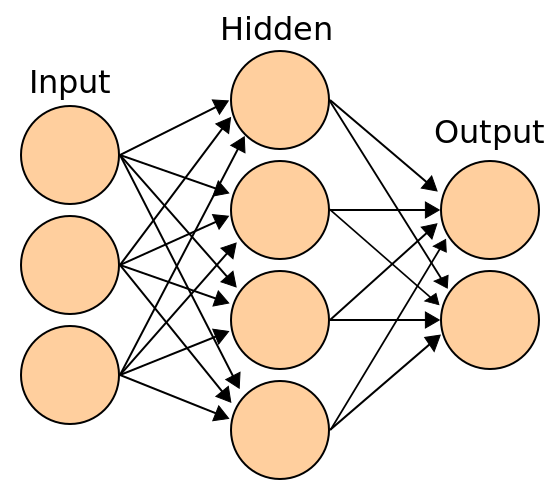
\includegraphics[width=\linewidth]{images/neural_network.png}
	\end{figure}
\end{columns}
\end{frame}

%------------------------------------------------

\begin{frame}{Backpropagation}

For one layer we have:
\begin{align}
y(x) = f(z(x)) \qquad z(x) = W x 
\end{align}
Derivatives with respect to the parameters W and the activations x:
\begin{align}
\frac{d y} { d W} &= \frac{ d y} {d z} \cdot \frac{d z} {d W} = f'(z(x)) \cdot \frac{d z} { d W} = f'(Wx) \cdot x^T \\
\frac{d y} { d x} &= \frac{ d y} {d z} \cdot \frac{d z} {d x} = f'(z(x)) \cdot \frac{d z} { d x} = f'(Wx) \cdot W
\end{align}

\end{frame}

%------------------------------------------------

\begin{frame}{Backpropagation}

For two layers we assume they have the same activation function $f$:
\begin{align}
y^{(1)}(x) &= f(z^{(1)}(x)) \quad && z^{(1)}(x) = W^{(1)} x \\
y^{(2)}(x) &= f(z^{(2)}(x)) \quad && z^{(2)}(x) = W^{(2)} x^{(2)} = W^{(2)} y^{(1)}
\end{align}
The derivatives within one layer are the same:
\begin{align}
\frac{d y^{(i)}} { d W^{(i)}} = f' (W^{(i)} x^{(i)}) \cdot x^{(i) T} \qquad
\frac{d y^{(i)}} { d x^{(i)}} = f'(W^{(i)} x^{(i)}) \cdot W^{(i)}
\end{align}
Across two layers we get:
\begin{align}
\frac{d y^{(2)}} { d W^{(1)}} &= \frac{ d y^{(2)}} {d y^{(1)}} \cdot \frac{d y^{(1)}} {d W^{(1)}} = 
\frac{ d y^{(2)}} {d x^{(2)}} \cdot \frac{d y^{(1)}} {d W^{(1)}}  \\
\frac{d y^{(2)}} { d x^{(1)}} &= \frac{ d y^{(2)}} {d y^{(1)}} \cdot \frac{d y^{(1)}} {d x^{(1)}} = 
\frac{ d y^{(2)}} {d x^{(2)}} \cdot \frac{d y^{(1)}} {d x^{(1)}}  
\end{align}
 
\end{frame}

%---------------------------------------------

\begin{frame}{Backpropagation}

Derivative across $N$ layers is :
\begin{align}
\frac{d y^{(N)}} { d W^{(1)}} &= \frac{ d y^{(N)}} {d x^{(N )}} \cdot \ldots \cdot \frac{ d y^{(2)}} {d x^{(2)}} \cdot \frac{d y^{(1)}} {d W^{(1)}}
\end{align}
 Why is it called Backpropagation?
\begin{align}
\frac{d y^{(N)}} { d W^{(2)}} = \underbrace{\frac{ d y^{(N)}} {d x^{(N )}} \cdot \ldots \cdot \frac{ d y^{(3)}} {d x^{(3)}}}_{ =: u^{(2)}}
\cdot \frac{d y^{(2)}} {d W^{(2)}}
= u^{(2)} \cdot \frac{d y^{(2)}} {d W^{(2)}}
\end{align}
From the perspective of layer $2$,  $u^{(2)} $ is the derivative that comes from up front. And the components are travelling backwards.
\end{frame}

%------------------------------------------------
\section{Issues during the Training Process}
%---------------------------------------------

\begin{frame}{Problem Setup}
	\begin{columns}
		\column{0.5\textwidth}
		This is the \href{https://github.com/zalandoresearch/fashion-mnist}{\color{blue}{Fashion MNIST dataset}}
			 \begin{itemize}
				\item  contains of $70000$ cloth items
				\item one picture and one label per item, i.e. "Dress", "Sneaker", "Coat"
				\item each picture is gray-scaled and $28$ x $28$ pixels
				\item example use case for now
				\item similar to classifying bacteria
				\item complex problem needs a more complex deeper network
			\end{itemize}
		\column{0.5\textwidth}
			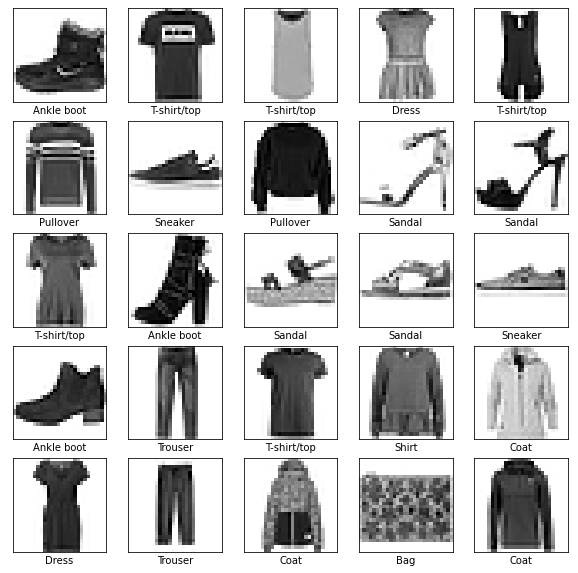
\includegraphics[width=\linewidth]{images/fashion_mnist.png}
	\end{columns}

\end{frame}

%---------------------------------------------

\begin{frame}{Example}
Let's oversimplify:
\begin{itemize}
\item each layer consists of one neuron
\item the derivative of each layer is $\frac{d y^{(i)} } {d x^{(i)}} = c $ constant
\item we have $N=10$ layers
\end{itemize}
What happens to the derivative of the first layer parameters $ W^{(1)} $?
\begin{align*}
\frac{d y^{(10)}} { d W^{(1)}} &= \frac{ d y^{(10)}} {d x^{(10 )}} \cdot \ldots \cdot \frac{ d y^{(2)}} {d x^{(2)}} \cdot \frac{d y^{(1)}} {d W^{(1)}} \\
 & = c \cdot \ldots \cdot c \cdot \frac{d y^{(1)}} {d W^{(1)}}
\end{align*}
\end{frame}


%------------------------------------------------

\begin{frame}{Vanishing / Exploding Gradient Problem}
\begin{align*}
\frac{d y^{(N)}} { d W^{(1)}} = c^{N -1} \cdot \frac{d y^{(1)}} {d W^{(1)}}
\end{align*}

For a huge number of layers $N$:
\begin{itemize}
\item $\frac{d y^{(N)}} { d W^{(1)}} $ get really big for $c > 1$
\item for $ c \approx 1 $ the derivative $\frac{d y^{(N)}} { d W^{(1)}}  \approx  \frac{d y^{(1)}} { d W^{(1)}} $
\item when $ c < 1 $ the gradient vanishes $ \frac{d y^{(N)}} { d W^{(1)}} \approx 0$
\end{itemize}
For more general cases of multiplying the Jacobians
\begin{align*}
\frac{d y^{(N)}} { d W^{(1)}} &= \frac{ d y^{(N)}} {d x^{(N )}} \cdot \ldots \cdot \frac{ d y^{(2)}} {d x^{(2)}} \cdot \frac{d y^{(1)}} {d W^{(1)}}
\end{align*}
the largest eigenvalues determine the convergence behavior. 

\end{frame}

%------------------------------------------------
\section{Self-normalizing Neural Networks (SNNs)}

\begin{frame}{Setup}
\begin{columns}[t]
\column{0.5 \textwidth}
	Let us look at one layer:
	\begin{itemize}
	\item $ y(x) = f(W x ) $ 
	\item $x \in \mathbb{R}^{n}$ activations current layer
	\item $y \in \mathbb{R}^{m}$ activations next layer
	\item $W \in  \mathbb{R}^{m \times n}$
	\item $f \in C^{0} $ continous non-linear function
	\end{itemize}
\column{0.5 \textwidth}	

	\begin{itemize}
	\item mean of the activations $ \mu = \mathbb{E}(x_i)$
	\item variance of the activations $ \nu = \text{Var} (x_i) $
	\item let $w^i$ be the i-th row of $W$
	\item the mean of the i-th row weights is $\omega^i := \sum_{j} w_{i j} $
	\item accordingly the second moment $\tau^i := \sum_{j} w_{i j}^2$
	\end{itemize}

\end{columns}

\end{frame}

%------------------------------------------------
\begin{frame}{Definition SNN}

How do mean $\mu$ and variance $\nu$ of the activations change to the next layer?
\begin{align*}
\begin{pmatrix} \mu \\  \nu \end{pmatrix}
\mapsto 
\begin{pmatrix} \tilde{\mu} \\  \tilde{\nu} \end{pmatrix}
= g \begin{pmatrix} \mu \\  \nu \end{pmatrix}
\end{align*}


\textbf{Definition}
\\
A neural network is called \textbf{self-normalizing} if there is a domain 
$ \Omega = \{ (\mu, \nu) \in \mathbb{R} \mid \mu \in [\mu_{\min}, \mu_{\max}], \nu \in [\nu_{\min}, \nu_{\max}] \} $ and a mapping $ g: \Omega \rightarrow \Omega$ such that
\begin{itemize}
\item $g(\Omega) \subset \Omega $ is a contraction
\item $g$ has a stable and attracting fixpoint $( \mu^*, \nu^*) \in \Omega $
\end{itemize}



\end{frame}

%------------------------------------------------

\begin{frame}{Self-normalizing map}


\begin{figure}[h!]
	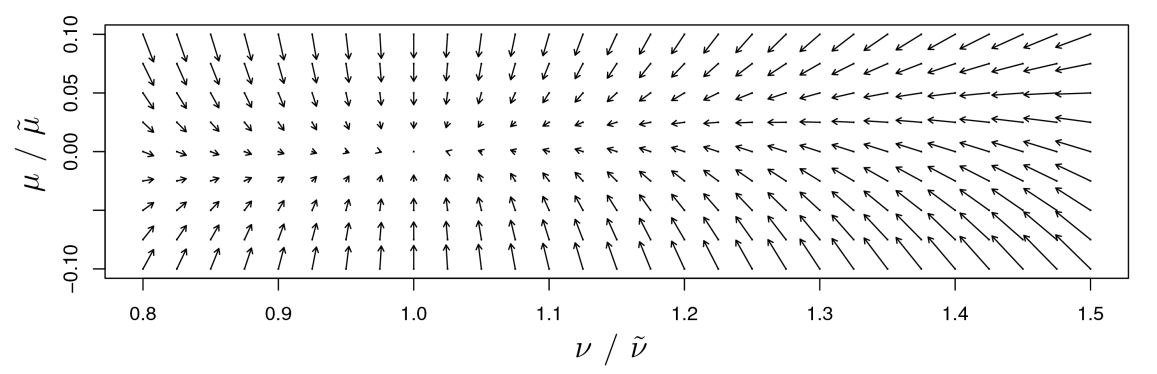
\includegraphics[width=\linewidth]{images/snn_map.png}
	\caption{Assuming the weight of each row $w^i$ to be normalized ($\omega = 0, \tau = 1$), we observe an attracting 		fixpoint $( \mu^* = 0, \nu^* =1) $. We need to pick the activation function accordingly.}
	\end{figure}

\end{frame}
%------------------------------------------------

\begin{frame}{Constructing a Self-normalizing Neural Network}
\begin{columns}
\column{0.5 \textwidth}
The key component to a SNN is to pick the activation function $f(x)$ to be
\begin{align}
\text{selu}(x) = \lambda
\begin{cases} 
      x & x\geq 0 \\
      \alpha ( e^x - 1) & x < 0
   \end{cases}
\end{align}
a \textbf{scaled exponential linear unit}
\\
Assuming 
\begin{itemize}
\item normalized weights: $\omega = 0, \tau = 1$ 
\item $z(x)$ to be normally distributed
\end{itemize}
specifies $ \alpha \approx 1.6733 $ and $ \lambda \approx 1.0507 $. 
\column{0.5 \textwidth}
	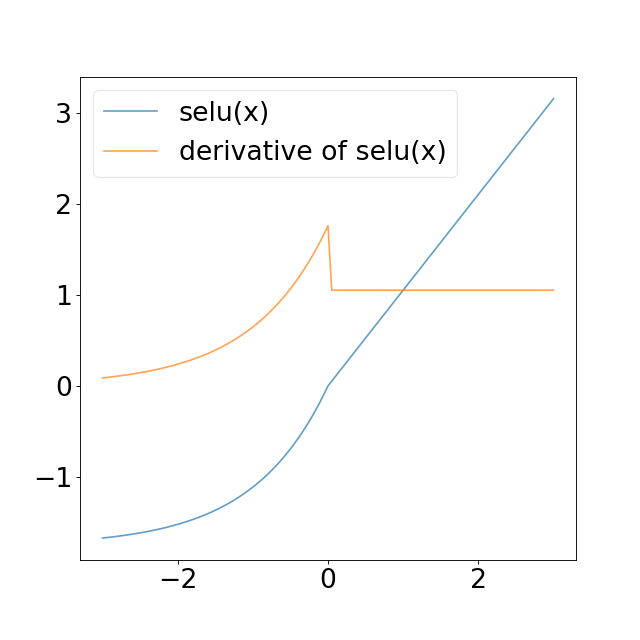
\includegraphics[width=\linewidth]{images/selu.png}
\end{columns}

\end{frame}


%------------------------------------------------
\begin{frame}{Why does that help?}
\begin{itemize}
\item supports deeper fully connected neural networks
\item matches a weight initialization of $\omega = 0$ and $ \tau = 1 $ very well 
\item automatically normalizes the activations of each layer
\begin{itemize}
\item $y^{(n)} \circ y^{(n - 1)} \circ \ldots \circ y^{(1)}(x^{(1)}) $ with normalized input features $x^{(1)}$
\item $y^{(n)} \circ y^{(n - 1)} \circ \ldots \circ y^{(k)}(x^{(k)}) $ with normalized activations $x^{(k)}$
\end{itemize}
\item prevents the gradient from exploding
\begin{itemize}
\item derivative of $\text{selu}(x) $ is highly bounded
\item extreme activations are damped by the convergence to $(\mu, \nu) = (0, 1)$
\end{itemize}
\item guarantees non vanishing gradients
\end{itemize}

\end{frame}


%------------------------------------------------

\begin{frame}[focus]
	Thank you \\
	Questions?
	\vfill
	\href{https://github.com/spirousschuh/presentations/blob/master/paper_slides/self-normalizing_nns/slides.pdf}
		{\small{Link to Slides}}




\end{frame}

%----------------------------------------------------------------------------------------
%	 CLOSING/SUPPLEMENTARY SLIDES
%----------------------------------------------------------------------------------------

\begin{frame}

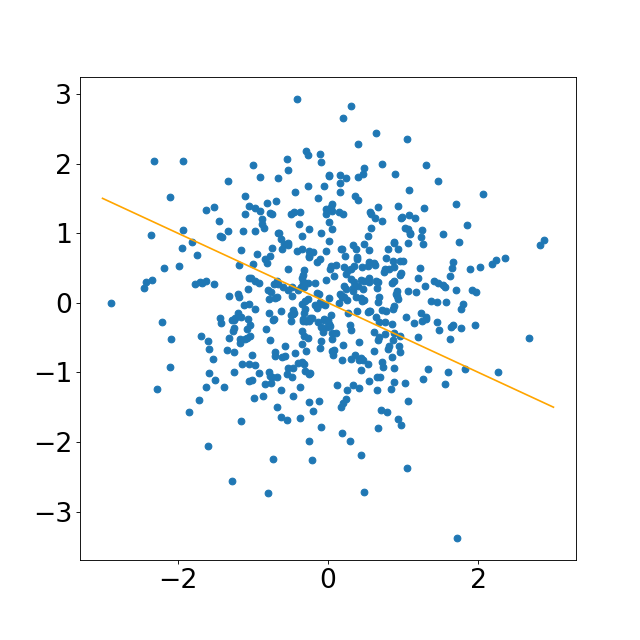
\includegraphics[width=0.6 \linewidth]{images/point_cloud.png}

\end{frame}


\appendix

\begin{frame}{References}
	\nocite{*} % Display all references regardless of if they were cited
	\bibliography{bibliography}
	\bibliographystyle{plain}
\end{frame}

%------------------------------------------------
\end{document}
